\documentclass[a4paper]{scrartcl}
\usepackage{url}
\usepackage{graphicx}
\graphicspath{ {Img/} }
\usepackage{float}

%\setkomafont{disposition}{\mdseries\rmfamily} %Unbolds title
\setkomafont{disposition}{\bfseries} %Serif font
\setkomafont{subtitle}{\rmfamily} %Unbold subtitle
\setkomafont{section}{\bfseries} %Bolded sections
\setkomafont{subsection}{\bfseries} %Bolded sections

%\renewcommand*{\thesection}{Problem~\arabic{section}} %"Problem" prefix to sections
%\renewcommand*{\thesubsection}{\alph{subsection}} %Letter subsectioning

\RedeclareSectionCommand[afterskip=-.5em]{subsection} %No after-subsection linebreak


\title{DirectX Term Project}
\subtitle{GMNG 4310}
%\date{2013-09-01}
\author{Jace Regenbrecht, Eduardo Brilanti, Aaron Cardinale, Juan Esparza}


\begin{document}
\maketitle

\section{Member responsibilities}

\subsection{Eduardo Brilanti.} Provided model and texture work for the title crawl text and rebel cruiser.
\subsection{Aaron Cardinale.} Provided model work for the star destroyer and blaster shots.
\subsection{Juan Esparza.} Implemented audio code work and provided files for intro music and explosion sound effect.
\subsection{Jace Regenbrecht.} Designed code base utilized by group, provided blaster audio and background texture work to project.

\section{Application description}

\begin{figure}[H]
\centering

\includegraphics[width=0.32\columnwidth]{DirectXTP1.png}
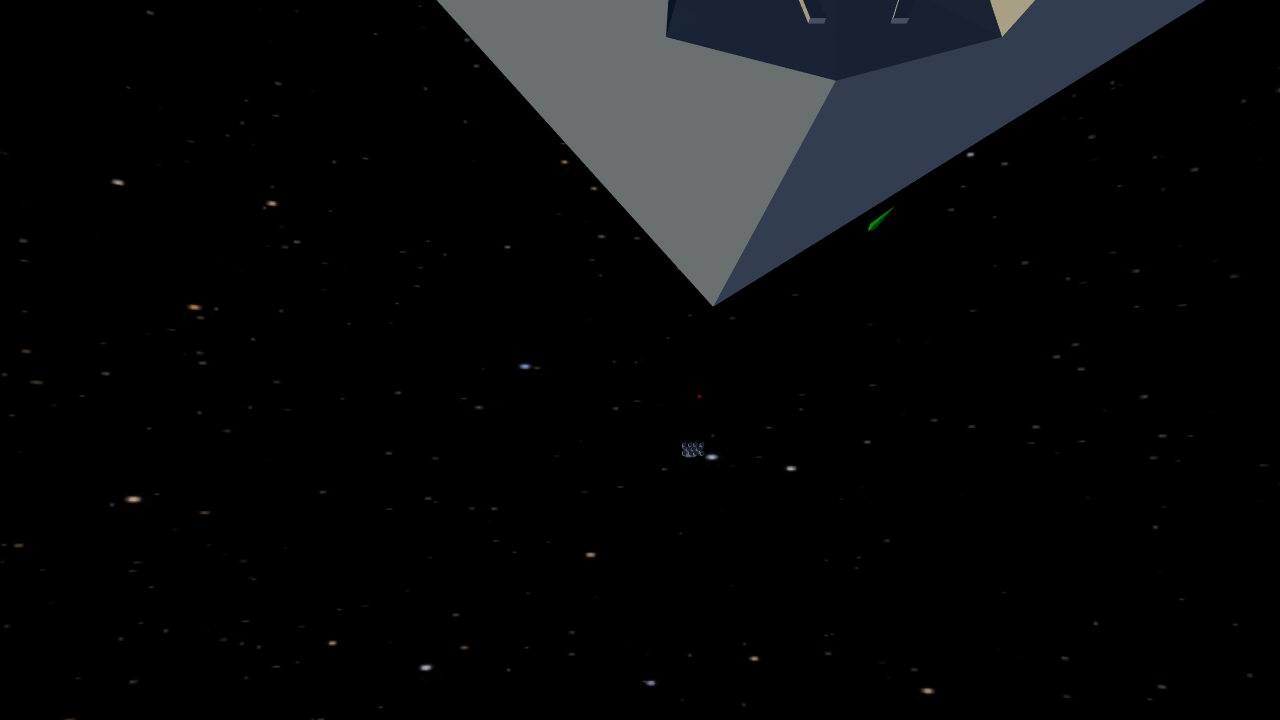
\includegraphics[width=0.32\columnwidth]{DirectXTP2.png}
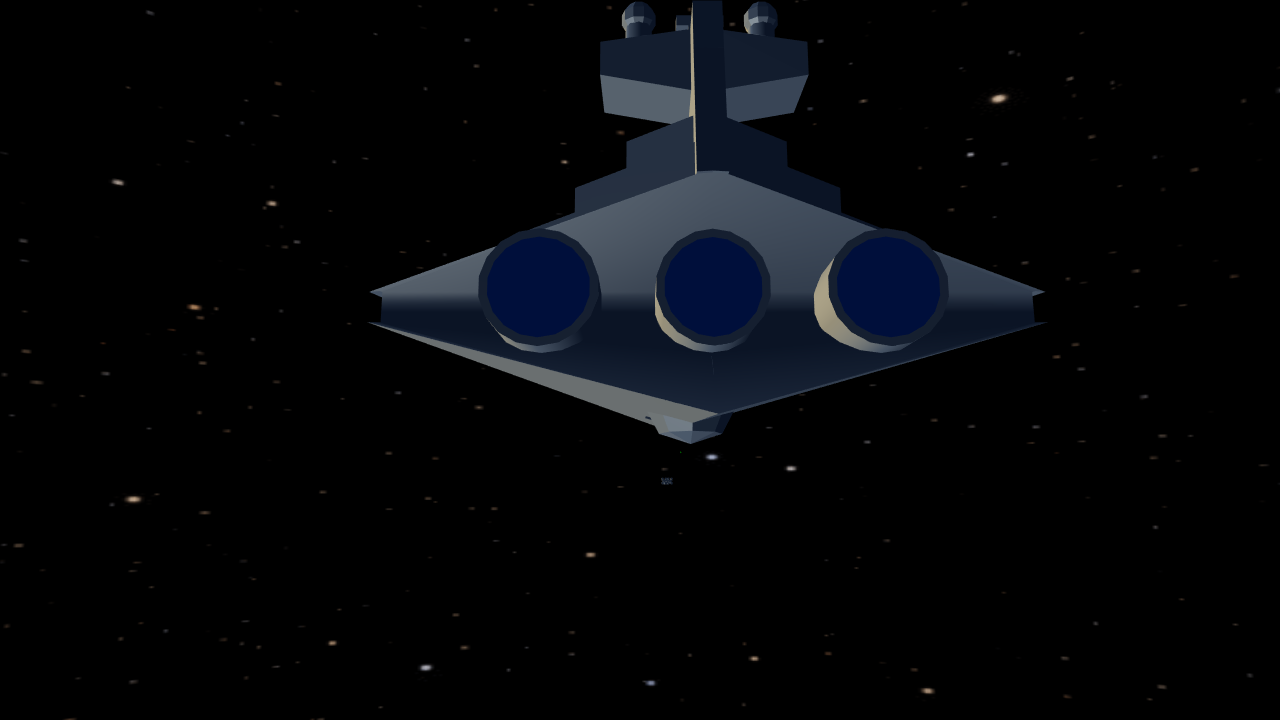
\includegraphics[width=0.32\columnwidth]{DirectXTP3.png}
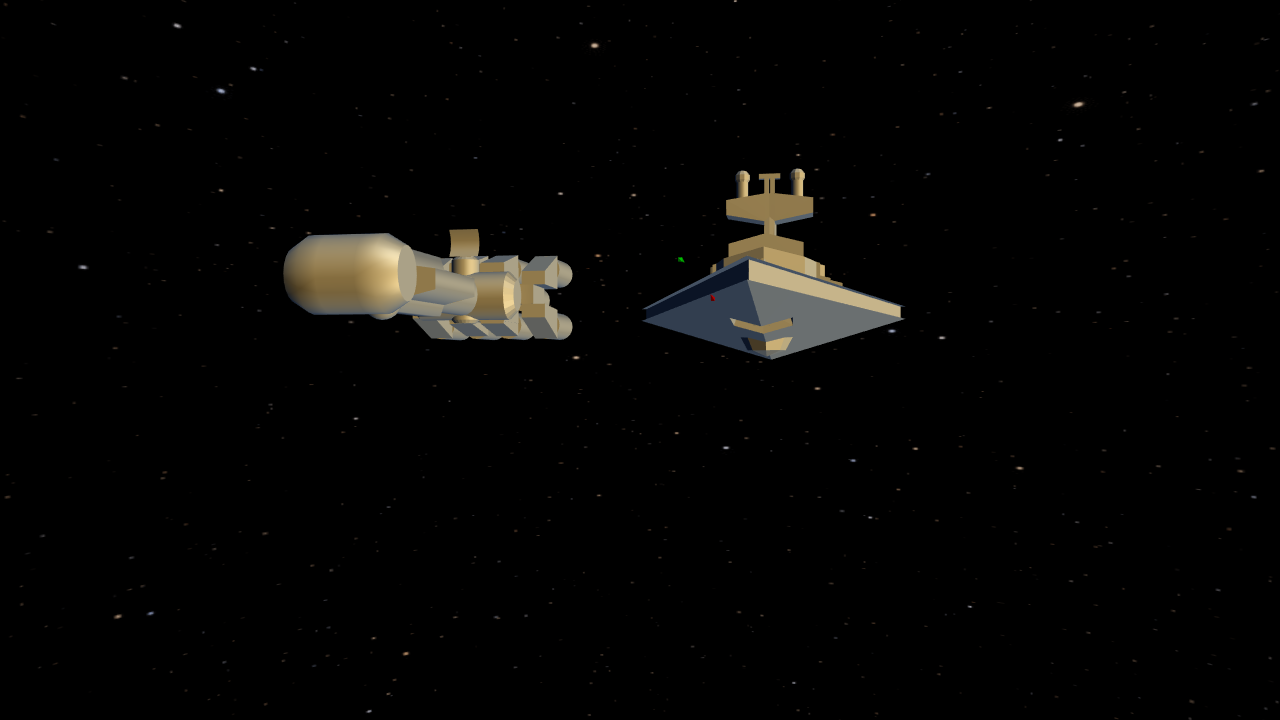
\includegraphics[width=0.32\columnwidth]{DirectXTP4.png}
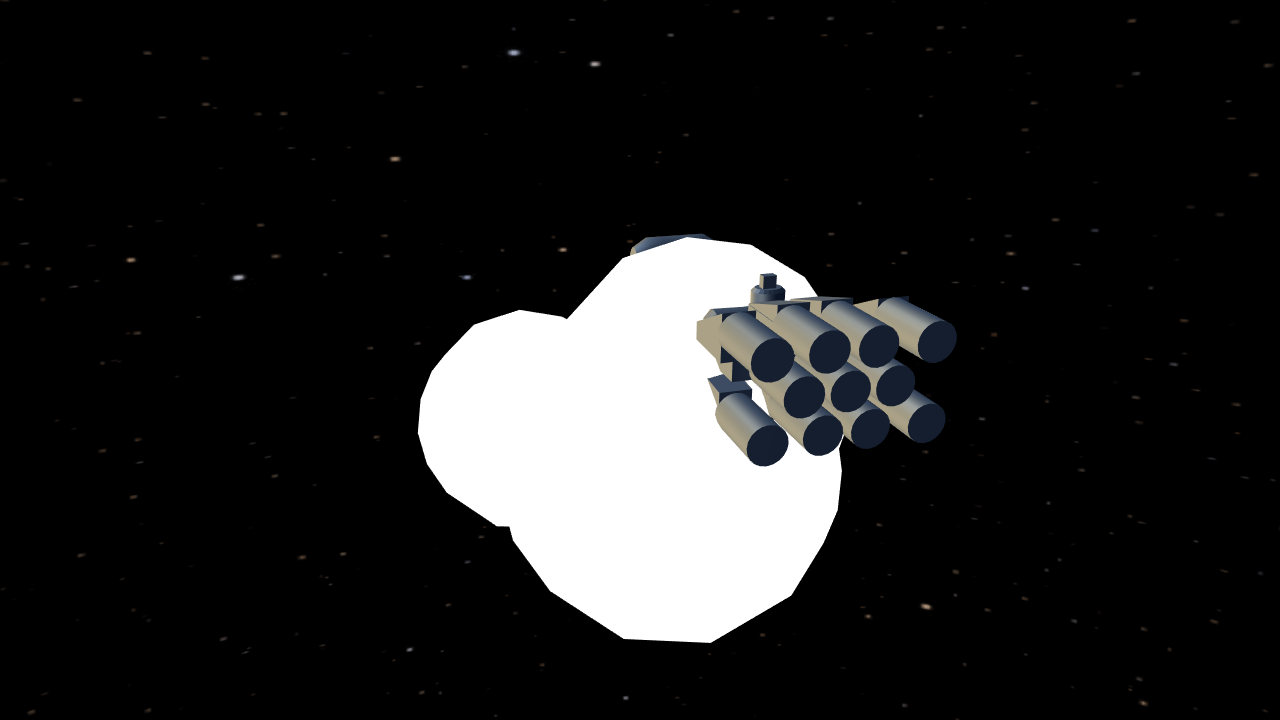
\includegraphics[width=0.32\columnwidth]{DirectXTP5.png}
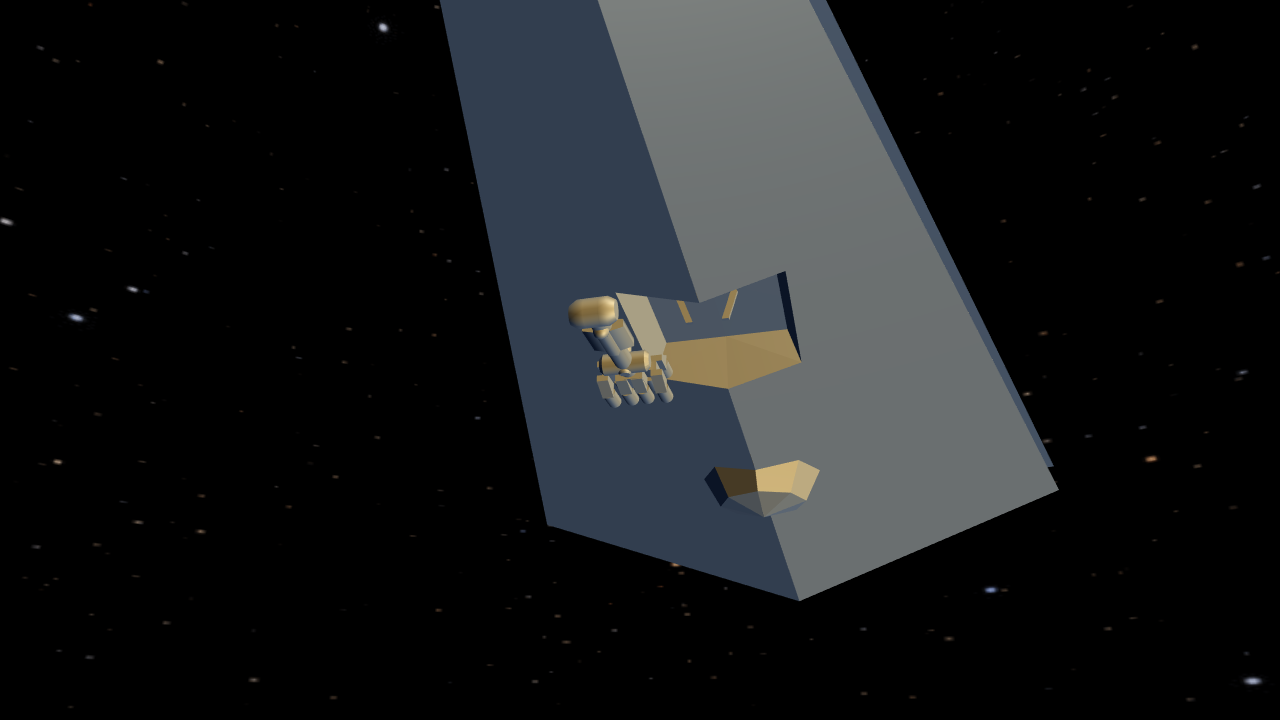
\includegraphics[width=0.32\columnwidth]{DirectXTP6.png}
\end{figure}

Our application is a two-minute short animation recreating the Star Wars: A New Hope opening scene. The animation opens with the famous Star Wars title crawl before panning down at the 1-minute mark to reveal the ensuring chase scene. Around the two minute mark the scene switches to a closeup of the rebel cruiser being disabled by a shot from the star destroyer, allowing it to be captured and ending the animation.

\section{Program status}

Program has no known runtime issues and has been built and run in multiple Windows 10 environments using Visual Studio 2015 without issue. Only issues with compilation may arise in environments running Windows versions earlier than Windows 8, as the project utilizes XAudio 2.8 for it's DirectX audio implementation.

\section{Code breakdown}

Our project utilizes the Microsoft's DirectX Tool Kit\cite{directxtk} library used in the labs, providing a useful set of classes to simplify the use of more complicated DirectX features. In addition, Chuck Walbourn's DirectX Visual Studio Templates\cite{d3dtemplate} was used as template code for the project, providing pre-completed window draw and update functions and thereby allowing us to focus on developing our project's DirectX infrastructure. Overall, our project includes around 750 lines of custom code with most work being done in the Game.h and Game.cpp files, plus the addition of completely custom files Maths.h, BlasterFlash.h, BlasterFlash.cpp, Blaster.h and Blaster.cpp.

Majority of the work done in the Game.h header is that addition of multiple objects and variables past line 75. In Game.cpp most of the game logic is handled in the Game::Update function with our custom code ranging between lines 68 and 290. Our render and drawing work is done in the Game::Render function between lines 306 and 373, with object creation and configuration being handled in the Game::CreateDevice function between lines 543 and 708. Additional setup work is also done in the Game::CreateResources function between lines 832 and 866. Some additional logic was also added to the Game:OnDeviceLost function between lines 873 and 899.

\section{Acknowledgments}
The DirectX tool Kit GitHub wiki\cite{directxtkwiki} was instrumental in providing the much-needed documentation that helped to make make this project possible. It's concise tutorials and thorough documentation are what ultimately led to the choice of DirectXTK as our DirectX library of choice over OGRE 3D.

\flushleft
\bibliographystyle{plain}
\bibliography{Writeup}

\end{document}

